\documentclass[aspectratio=169]{beamer}

% --- Theme Configuration ---
\usetheme{Madrid}
\usecolortheme{whale}
\setbeamercolor{titlelike}{parent=structure,bg=blue!80!black,fg=white}

% --- Packages ---
\usepackage{graphicx}
\usepackage{booktabs}
\usepackage{hyperref}
\usepackage{tikz}
\usetikzlibrary{shadows, positioning, arrows}
\usepackage{tcolorbox}

% --- Title Information ---
\title[Instrunet AI]{INSTRUNET AI}
\subtitle{Deep Learning for Music Instrument Recognition}
\author{Jagath Kiran}
\date{January 23, 2026}

\begin{document}

% 1. Title Slide
\begin{frame}[plain]
    \titlepage
\end{frame}

% 2. Table of Contents
\begin{frame}{Agenda}
    \tableofcontents
\end{frame}

% 3. Problem Statement
\section{Problem Statement}
\begin{frame}{Problem Statement}
    \centering
    \vspace{1.5cm}
    \Large
    "Identifying instruments in music tracks is crucial for indexing and recommendation. However, manual labeling is time-consuming, error-prone, and impossible to scale for massive digital libraries."
\end{frame}

% 4. Data Engineering (Replaces Timeline)
\section{Data Engineering}
\begin{frame}{Data Engineering \& Preprocessing}
    \begin{columns}
        \column{0.5\textwidth}
        \textbf{Preprocessing Pipeline:}
        \begin{itemize}
            \item \textbf{Standardization:} All audio resampled to \textbf{16kHz Mono}.
            \item \textbf{Silence Removal:} Energy-based filtering to remove non-musical segments.
            \item \textbf{Windowing:} 3.0s segments with 50\% overlap.
        \end{itemize}
        
        \vspace{0.3cm}
        \textbf{Augmentation (SpecAugment):}
        \begin{itemize}
            \item Random \textbf{Time Masking} (Vertical blocks).
            \item Random \textbf{Frequency Masking} (Horizontal blocks).
        \end{itemize}

        \column{0.5\textwidth}
        \centering
        \includegraphics[width=0.9\textwidth]{../../outputs/frontend/dashboard_audio_spectrogram.png} \\
        \tiny{Generated Mel-Spectrogram}
    \end{columns}
\end{frame}

% 5. System Architecture (Enhanced)
\section{System Architecture}
\begin{frame}{System Architecture: End-to-End Pipeline}
    \centering
    \resizebox{0.95\textwidth}{!}{
    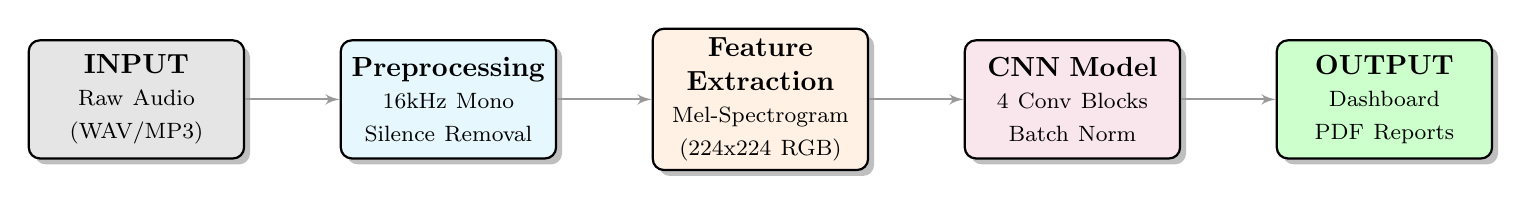
\begin{tikzpicture}[
        node distance=1.5cm and 1.2cm,
        auto,
        thick,
        block/.style={rectangle, draw, fill=blue!10, text width=2.5cm, text centered, rounded corners, minimum height=1.5cm, drop shadow},
        line/.style={draw, -latex', thick, gray!80}
    ]
        % Nodes
        \node [block, fill=gray!20] (input) {\textbf{INPUT}\\[2pt]\footnotesize Raw Audio\\(WAV/MP3)};
        \node [block, right=of input, fill=cyan!10] (pre) {\textbf{Preprocessing}\\[2pt]\footnotesize 16kHz Mono\\Silence Removal};
        \node [block, right=of pre, fill=orange!10] (feat) {\textbf{Feature Extraction}\\[2pt]\footnotesize Mel-Spectrogram\\(224x224 RGB)};
        \node [block, right=of feat, fill=purple!10] (cnn) {\textbf{CNN Model}\\[2pt]\footnotesize 4 Conv Blocks\\Batch Norm};
        \node [block, right=of cnn, fill=green!20] (out) {\textbf{OUTPUT}\\[2pt]\footnotesize Dashboard\\PDF Reports};

        % Edges
        \path [line] (input) -- (pre);
        \path [line] (pre) -- (feat);
        \path [line] (feat) -- (cnn);
        \path [line] (cnn) -- (out);
    \end{tikzpicture}
    }
    
    \vspace{0.5cm}
    \hrule
    \vspace{0.3cm}
    
    \begin{columns}
        \column{0.33\textwidth}
        \textbf{Feature Extraction:}
        \begin{itemize}
            \item \textbf{Input:} Mel-Spectrograms treat audio as images.
            \item \textbf{Why?} Captures harmonic textures better than waveforms.
        \end{itemize}
        
        \column{0.33\textwidth}
        \textbf{Model Design:}
        \begin{itemize}
            \item \textbf{Backbone:} 4-Layer CNN.
            \item \textbf{Regularization:} Spatial Dropout \& L2.
            \item \textbf{Goal:} Shift-invariant detection.
        \end{itemize}
        
        \column{0.33\textwidth}
        \textbf{Inference Logic:}
        \begin{itemize}
            \item \textbf{Method:} Sliding Window.
            \item \textbf{Aggregation:} Mean probability across all windows.
        \end{itemize}
    \end{columns}
\end{frame}% 6. Dataset & Performance
\section{Dataset \& Performance}
\begin{frame}{Dataset \& Model Performance}
    \begin{columns}
        \column{0.45\textwidth}
        \textbf{Supported Classes (11):}
        \footnotesize
        \begin{itemize}
            \item \textbf{Strings:} Cello, Violin, Acoustic Guitar, Electric Guitar
            \item \textbf{Winds:} Clarinet, Flute, Saxophone, Trumpet
            \item \textbf{Keys/Other:} Piano, Organ, Human Voice
        \end{itemize}
        
        \vspace{0.3cm}
        \textbf{Key Metrics:}
        \begin{itemize}
            \item \textbf{Overall Accuracy:} \textbf{82.24\%}
            \item \textbf{Best Class:} Voice (F1: 0.92)
            \item \textbf{Challenging:} Violin (F1: 0.71)
        \end{itemize}

        \column{0.55\textwidth}
        \centering
        \includegraphics[width=0.95\textwidth]{../../outputs/normalized_confusion_matrix.png} \\
        \tiny{Normalized Confusion Matrix}
    \end{columns}
\end{frame}

% 7. Demo Flow
\section{Control Flow}
\begin{frame}{Control Flow: 3-Step Process}
    \begin{enumerate}
        \item \textbf{AUTHENTICATE:} Secure login to track history and save analysis results.
        \item \textbf{ANALYZE:} Upload local files or record live audio. The system generates real-time visual spectrograms.
        \item \textbf{EXPORT:} Review class probabilities and download a professional PDF/JSON summary report.
    \end{enumerate}
    \vspace{0.3cm}
    \centering
    \includegraphics[width=0.4\textwidth]{../../outputs/frontend/dashboard_initial.png}
\end{frame}

% 8. Demo Screenshots
\section{Demo Screenshots}
\begin{frame}{User Interface \& Analytics}
    \begin{columns}
        \column{0.5\textwidth}
        \centering
        \includegraphics[width=0.9\textwidth]{../../outputs/frontend/login_page.png} \\
        \textbf{\\Secure Authentication}
        
        \column{0.5\textwidth}
        \centering
        \includegraphics[width=0.9\textwidth]{../../outputs/frontend/dashboard_predictions.png} \\
        \textbf{\\Instrument Probability Analytics}
    \end{columns}
\end{frame}

% 9. Future Scope & Conclusion
\section{Extensions}
\begin{frame}{Future Scope \& Conclusion}
    \begin{itemize}
        \item \textbf{Polyphony:} Expanding to Multi-Label detection for complex orchestral tracks.
        \item \textbf{Stem Separation:} Isolating the detected instrument for remixing.
        \item \textbf{Conclusion:} Instrunet AI delivers a production-ready pipeline for automated instrument identification.
    \end{itemize}
    \vspace{0.5cm}
    \centering
    \textit{"Instrunet AI: Turning sound into structured information."}
\end{frame}

% 10. Thank You
\begin{frame}[plain]
    \centering
    \Huge{\textbf{THANK YOU}} \\
    \vspace{1cm}
    \large{Questions?}
\end{frame}

\end{document}
